\chapter{Les projets}
La gestion des clients associe à chacun d'eux un ou plusieurs projets : il est donc nécessaire de visualiser la liste des projets pour chacun des clients. 
\begin{figure}[H]
	\centering
	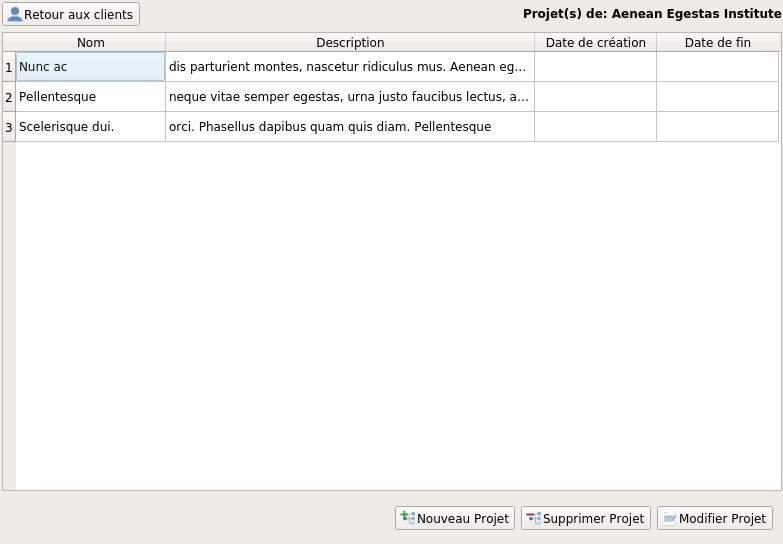
\includegraphics[width=12cm]{screens/projets.png}
	\caption{Gestion des projets d'un client}
\end{figure}

\section{Liste des projets\index{Projet!Liste}}
%La liste des clients, cf. figure 3.1, est accessible dès l’ouverture du logiciel. Celle-ci se trouve au centre du logiciel. 

%La liste des clients contient uniquement les informations permettant de facilement les identifier à savoir, le nom de la société, le nom, prénom, le numéro de téléphone et l’adresse e-mail. La sélection dans le tableau de l’un des clients permet, via le panneau du client, d’obtenir les informations détaillées sur celui-ci. 

\section{Ajout d'un client\index{Projet!Ajouter}}
%L'ajout d’un patient peut se faire via le menu <<Client $\rightarrow$ Nouveau Client>>, via la barre d'outils ou encore via le bouton situé sous la
liste. 
\begin{figure}[H]
	\centering
	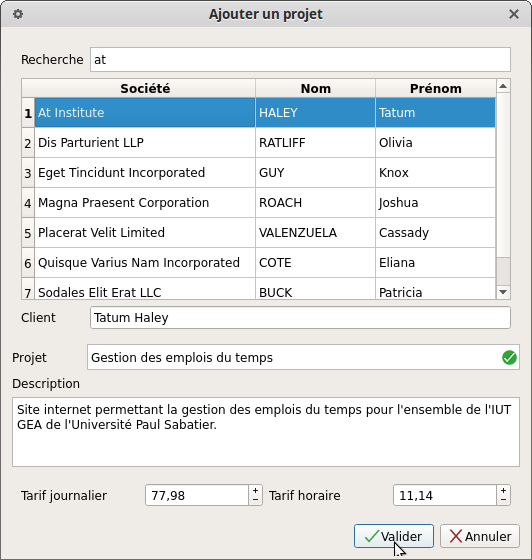
\includegraphics[width=7cm]{screens/ajouterProjet.png}
	\caption{Ajouter un client}
\end{figure}

\section{Édition d'un client\index{Projet!Éditer}}
 %L’édition d’un client a pour but de corriger d’éventuelles erreurs sur les informations d’un client. Pour ce faire, il suffit de sélectionner un client dans le tableau et de cliquer sur le bouton <<Modifier>> situé sous la liste des clients. Il est aussi possible de faire un clic droit sur le client dans le tableau puis, via le menu contextuel, d'"Éditer le client". 
% La fenêtre est similaire à celle lors d’un ajout de client, seul diffère les champs qui sont pré-remplis. 
\begin{figure}[H]
	\centering
	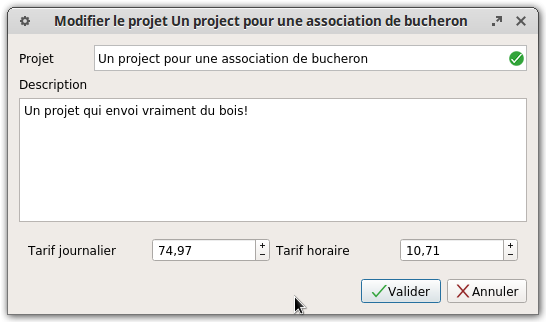
\includegraphics[width=7cm]{screens/editerProjet.png}
	\caption{Ajouter un client}
\end{figure}